\documentclass[../../../../main.tex]{subfiles}

\begin{document}

\section*{第1問}

\begin{proof}[解]
\begin{itemize}
  \item[(i)] $a^2-2b^2=\pm1\ \cdots *$
  \item[(ii)] $a+\sqrt2\,b>0$
\end{itemize}
$p=1+\sqrt2$とおく。$1^2-2\cdot1^2=-1$から，$p\in G$である。

\textbf{(1)} $1<g<p$をみたす$G$の要素$g$があると仮定すると，
\[
1<a+\sqrt2b<1+\sqrt2 \quad\cdots\text{①}
\]

\textbf{⑦ $a-\sqrt2b>0$の時}

(ii)から，$a^2-2b^2=(a+\sqrt2b)(a-\sqrt2b)>0$だから(i)から，$a^2-2b^2=1$である。①から
\[
a-\sqrt2b<1<(1+\sqrt2)(a-\sqrt2b)
\]
\[
-1+\sqrt2<a-\sqrt2b<1 \quad\cdots\text{②}
\]
①②を辺々足して
\[
\frac{\sqrt2}{2}<a<1+\frac{\sqrt2}{2}
\]
$a\in\mathbb{Z}$から$a=1$で，①に代入して$0<\sqrt2b<\sqrt2$となり，$b\in\mathbb{Z}$に矛盾。

\textbf{⑦ $a-\sqrt2b<0$の時}

⑦と同様に$a^2-2b^2=-1$であって，①から
\[
(1+\sqrt2)(a-\sqrt2b)<-1<a-\sqrt2b
\]
\[
-1<a-\sqrt2b<1-\sqrt2 \quad\cdots\text{③}
\]
①③を辺々足して
\[
0<a<1
\]
これは$a\in\mathbb{Z}$に矛盾。

以上から，$1<g<p$をみたす$g\in G$は存在せず，$u=p=1+\sqrt2$である。

\textbf{(2)} 証明は帰納法による。$n=0$の時は$f(n)=gu^n$とおくと$f(0)=g\in G$だから成立するので，以下$n=k\ (\in\mathbb{Z})$での$f(k)\in G$を仮定し，$n=k\pm1$での成立を示す。$f(k)=\alpha+\sqrt2\beta$とおく。
\[
f(k+1)=f(k)\cdot u=(\alpha+\sqrt2\beta)(1+\sqrt2)=(\alpha+2\beta)+\sqrt2(\alpha+\beta)
\]
であり，$f(k)\in G$より$(\alpha,\beta)$が$*$をみたすことから，
\[
f(k+1)>0,\quad \alpha,\beta\in\mathbb{Z}
\]
\[
(\alpha+2\beta)^2-2(\alpha+\beta)^2=-\alpha^2+2\beta^2=\pm1
\]
となり，$f(k+1)\in G$。したがって，$n=k+1$でも成立。

又，
\[
f(k-1)=(\alpha+\sqrt2\beta)(1+\sqrt2)^{-1}=(\alpha+\sqrt2\beta)(-1+\sqrt2)=(-\alpha+2\beta)+\sqrt2(\alpha-\beta)
\]
より，$f(k-1)=f(k)(\sqrt2-1)>0$，$-\alpha+2\beta,\ \alpha-\beta\in\mathbb{Z}$，
\[
(-\alpha+2\beta)^2-2(\alpha-\beta)^2=-\alpha^2+2\beta^2=\pm1
\]
となって，$n=k-1$でも成立する。

以上から，$n=k\pm1$でも成立するから，示された。

\textbf{(3)} $G$の要素$g$があって，$g\ne u^n\ (n\in\mathbb{Z})$だと仮定する。

\textbf{[補題]} $(1+\sqrt2)^n=A_n+\sqrt2B_n,\ (1-\sqrt2)^n=A_n-\sqrt2B_n\ (A_n,B_n\in\mathbb{Z})$と表せることを示す。

\textbf{（証明）} $n=0$の時は明らか。まず$n\in\mathbb{N}$の時，2項展開から
\[
(1+\sqrt2)^n=(1+{}_nC_2\cdot2+\cdots)+\sqrt2({}_nC_1+{}_nC_3+\cdots)
\]
\[
(1-\sqrt2)^n=(1+{}_nC_2\cdot2+\cdots)-\sqrt2({}_nC_1+{}_nC_3+\cdots)
\]
であり，${}_nC_k\in\mathbb{Z}$だから[補題]は成立。$n\le-1\in\mathbb{Z}$の時，$n=-p\ (p\in\mathbb{N})$とおきかえ，$(1+\sqrt2)^{-1}=-1+\sqrt2,\ (1-\sqrt2)^{-1}=-1-\sqrt2$だから同様にして[補題]は成立。以上から示された。

したがって，$g\ne u^n$ならば$a-b\sqrt2\ne(1-\sqrt2)^n$である。辺々かけて
\[
a^2-2b^2\ne(1+\sqrt2)^n(1-\sqrt2)^n=(-1)^n
\]
これが任意の$n\in\mathbb{Z}$で成立するので，$a^2-2b^2\ne\pm1$だが，これは$g\in G$に矛盾。以上から，$g=u^n$とかけるから，$G$の任意の要素は$u^n$の形でかける。
\end{proof}

\newpage

\section*{第2問}

\begin{proof}[解]
\textbf{(1)} $t$にまって，切断面は変化する直方体の頂点を通る。$\pi(t): x+\dfrac12y+\dfrac13z=t$とおく。$V$の体積は$T=6$である $\cdots$①

\textbf{$1^\circ$ $0<t\le1$の時}

切断立体のうち，三角錐のものの体積は
\[
\frac13\cdot t\cdot\left(\frac12\cdot t\cdot 2t\cdot\frac{3}{2}\right)=t^3
\]
であり，これは$t\le3/2$より小さいから，$f(t)=t^3$

\textbf{$2^\circ$ $1\le t\le2$の時}

切断立体のうち，原点$O$を含む方の体積は，コーナーの三角錐を3つ分あわせて切り取ることになり，
\[
t^3-3(t-1)^3=-2t^3+9t^2-9t+3\equiv g(t)
\]
である。$g'(t)=-6(t^2-3t+2)=-6(t-2)(t-1)\ge0\ (1\le t\le2)$だから$g(t)$は非減少で，$g(3/2)=3$だから，
\[
f(t)=
\begin{cases}
g(t) & \left(1\le t\le\dfrac32\right) \\
6-g(t) & \left(\dfrac32\le t\le2\right)
\end{cases}
\]

\textbf{$3^\circ$ $2\le t<3$の時}

対称性から，$f(t)=(3-t)^3$

以上から
\[
f(t)=
\begin{cases}
t^3 & (0\le t\le1) \\
-2t^3+9t^2-9t+3 & \left(1\le t\le\dfrac32\right) \\
2t^3-9t^2+9t+3 & \left(\dfrac32\le t\le2\right) \\
(3-t)^3 & (2\le t\le3)
\end{cases}
\]

\textbf{(2)} $h(t)=t^3,\ P(t)=6-g(t)$とおく。以下$h\to0$と扱う。$f(t)$は各区間で連続である。

\textbf{⑦ $t=1$の時}
\[
\frac{f(1+h)-f(1)}{h}\xrightarrow{h\to0}g'(1)=3, \qquad \frac{f(1-h)-f(1)}{-h}\xrightarrow{h\to0}f'(1)=3
\]
より左右極限が一致し，微分可能。

\textbf{⑦ $t=3/2$の時}
\[
\frac{f(3/2+h)-f(3/2)}{h}\xrightarrow{h\to0}P'(3/2)=-\frac92, \qquad \frac{f(3/2-h)-f(3/2)}{-h}\xrightarrow{h\to0}g'(3/2)=+\frac92
\]
より左右極限が一致せず，微分不可。

以上から
\[
t=1:\ \text{possible}, \qquad t=\frac32:\ \text{impossible}
\]
\end{proof}

\newpage

\section*{第3問}

\begin{proof}[解]
円$O_k\ (k=1,2,\cdots,5)$の半径を$r_k$とすると，題意から
\[
r_1=1, \qquad r_2=a, \qquad r_3=r_4=\frac{1-a}{2}
\]
である。又，$\angle DAB=\theta$とおく（$0<\theta<\pi/2\ \cdots$①）。

\begin{center}
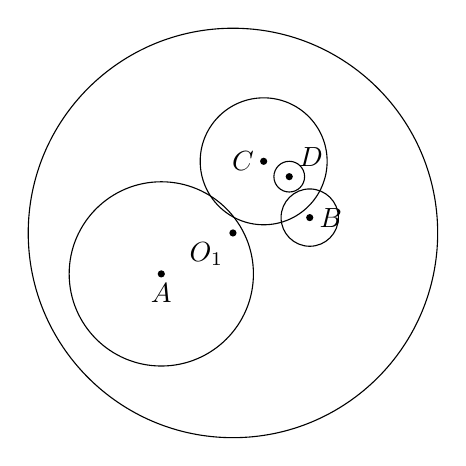
\begin{tikzpicture}[scale=1.3, >=stealth]
  \draw (0,0) circle (2);
  \draw (-0.7,-0.4) circle (0.9);
  \draw (0.3,0.7) circle (0.62);
  \draw (0.75,0.15) circle (0.28);
  \draw (0.55,0.55) circle (0.15);
  \fill (0,0) circle (1pt) node[below left] {$O_1$};
  \fill (-0.7,-0.4) circle (1pt) node[below] {$A$};
  \fill (0.3,0.7) circle (1pt) node[left] {$C$};
  \fill (0.75,0.15) circle (1pt) node[right] {$B$};
  \fill (0.55,0.55) circle (1pt) node[above right] {$D$};
\end{tikzpicture}
\end{center}

$O_3$と$O_4$の接点を$E$とする。$E$は$AD$，$BC$の交点であることに注意する。

\textbf{(1)} ピタゴラスの定理から
\[
AE=\sqrt{\left(a+\frac{1-a}{2}\right)^2-\left(\frac{1-a}{2}\right)^2}=\sqrt{a} \quad\cdots *
\]
\[
DE=\sqrt{\left(r_5+\frac{1-a}{2}\right)^2-\left(\frac{1-a}{2}\right)^2}=\sqrt{r_5^2+(1-a)r_5}
\]
したがって，$r_1=1$を2通りで表して
\[
1=AE+DE+r_5=\sqrt a+\sqrt{r_5^2+(1-a)r_5}+r_5
\]
\[
(1-\sqrt a)-r_5=\sqrt{r_5^2+(1-a)r_5}
\]
\[
r_5^2-2(1-\sqrt a)r_5+(1-\sqrt a)^2=r_5^2+(1-a)r_5 \quad\cdots\text{②}, \qquad (1-\sqrt a)-r_5\ge0\quad\cdots\text{③}
\]
②から
\[
r_5=\frac{(1-\sqrt a)^2}{2(1-\sqrt a)+(1-a)}=\frac{(1-\sqrt a)^2}{3-a-2\sqrt a}
\]
である。$t=\sqrt a\ (0<t<1,\ \cdots$④$)$とおいて③に代入
\[
(1-t)+\frac{(1-t)^2}{t^2+2t-3}=(1-t)-\frac{1-t}{t+3}=\frac{(1-t)(t+2)}{t+3}\ge0\quad(\because④)
\]
から，この$t$は③をみたして良い。この時，$*$から
\[
DE=\sqrt{\frac{1-t}{t+3}\left(\frac{1-t}{t+3}+1-t\right)}=\sqrt{\frac{(1-t)^2}{(t+3)^2}(t+2)^2}=\frac{(1-t)(t+2)}{t+3}\quad(\because④)
\]
\[
AE=t
\]
だから
\[
S(a)=\triangle ABD+\triangle ACD=AD\cdot BE=\left(t+\frac{(1-t)(t+2)}{t+3}\right)\cdot\frac{1-t^2}{2}
\]
\[
=\frac{(t+1)(1-t)}{t+3}\cdot\frac{(\sqrt a+1)(1-\sqrt a)}{\sqrt a+3}
\]

\textbf{(2)} $f(t)=\dfrac{(t+1)(1-t)^2}{t+3}$とおく。$f(t)$の$0<t<1$での最大値をもとめれば良い。

$p=t+3$とおくと，$3<p<4$で，
\[
f(t)=\frac{(p-2)^2(4-p)}{p}
\]
\[
\frac{df}{dp}=\frac{p[2(p-2)(4-p)-(p-2)^2]-(p-2)^2(4-p)}{p^2}=\frac{-2(p-2)(p^2-2p-4)}{p^2}
\]
より，下表をうる。
\begin{center}
\begin{tabular}{c|ccccc}
$p$ & $3$ & & $1+\sqrt5$ & & $4$ \\
\hline
$f'$ & & $+$ & $0$ & $-$ & \\
\hline
$f$ & & $\nearrow$ & & $\searrow$ &
\end{tabular}
\end{center}
したがって，$p=1+\sqrt5$で最大値$10\sqrt5-22$をとる。
\end{proof}

\newpage

\section*{第4問}

\begin{proof}[解]
$C$上の点$P(x,y)$での$C$の接線$\ell$が常に$Q\left(\dfrac{6x^3+1}{6x^2},2y\right)$を通る。
\[
\frac{6x^3+1}{6x^2}-x=\frac{1}{6x^2}\ne0
\]
から，直線$PQ$は$y$軸平行でないので，$XY$平面において，
\[
\ell: Y=\frac{dy}{dx}(X-x)+y
\]
と表せる。$Q$が$\ell$上にあるので，
\[
2y=\frac{dy}{dx}\left(\frac{6x^3+1}{6x^2}-x\right)+y
\]
\[
y=\frac{1}{6x^2}\frac{dy}{dx}
\]
\[
6x^2\,dx=\frac1y\,dy
\]
両辺積分して，定数$C_1$として
\[
2x^3+C_1=\log|y| \quad\cdots\text{①}
\]
$C$は連続だから，$(x,y)=(0,2)$でも①がなりたつので，
\[
C_1=\log2
\]
したがって，
\[
|y|=2\cdot e^{2x^3}
\]
\[
y=\pm2\cdot e^{2x^3}
\]
複号負は$C$が$(0,2)$を通ることに反するから，
\[
y=2e^{2x^3}
\]
\end{proof}

\newpage

\section*{第5問}

\begin{proof}[解]
3人を$a_1,a_2,a_3$とし，$a_1$の得点を確率変数$X$とする。

\textbf{Aの場合}

$X=k$となる確率$P(X=k)$は，$a_1$が$k$を引き，$a_2,a_3$が$k-1$以下の枚を引く場合。
\[
P(X=1)=0, \qquad P(X=k)=\frac{1}{n^3}(k-1)^2\quad(k=2,\cdots,n)
\]
他の場合の$a_1$の得点は0だから，
\[
E=\sum_{k=2}^n\frac{k}{n^3}(k-1)^2=\frac{1}{n^3}\sum_{k=2}^n\left\{k(k-1)(k-2)+k(k-1)\right\}
\]
\[
=\frac{1}{n^3}\left[\frac14(n+1)n(n-1)(n-2)+\frac13(n+1)n(n-1)\right]
\]
\[
=\frac{(n+1)(n-1)(3n-2)}{12n^2}
\]

\textbf{Bの場合}

$a_1$の引いた数が$Y_1$である時，$a_1$が得点するのは，$a_2,a_3$の引いた数$Y_2,Y_3$として，$Y_2,Y_3\le Y_1-1$の時。したがって，この時の$a_1$の得点の期待値$E(Y_1)$は，$Y_1=1$の時0，$Y_1\ge2$のとき，
\[
E(Y_1)=\frac{1}{n^3}\left(\text{条件をみたす全ての}(Y_2,Y_3)\text{についての}Y_2+Y_3\text{の和}\right)
\]
であるから
\[
E(Y_1)=\frac{1}{n^3}\cdot2(Y_1-1)\{1+\cdots+(Y_1-1)\}=\frac{1}{n^3}(Y_1-1)^2Y_1
\]
したがって，もとめる期待値$E'$は
\[
E'=\sum_{Y_1=1}^nE(Y_1)=\frac{1}{12n^2}(n+1)(n-1)(3n-2)
\]

よって，いずれの場合も
\[
\frac{1}{12n^2}(n+1)(n-1)(3n-2)
\]
\end{proof}

\end{document}
